% manuscript.tex -- publication-facing source of truth for manuscript v1 (D047).
% Provenance: every visible scientific number carries a trailing comment naming its authority:
%   N-xx  -> paper/PAPER_NUMERIC_CLAIMS.csv (built by paper/build_paper_numbers.py from frozen D041-D043 tables)
%   F-01  -> revision_v1/V1_NUMERIC_CLAIMS.csv (frame verification composition; scripts/build_manuscript_tables.py)
%   REL   -> D034 pre-adjudication reliability table (coding_reliability/reliability_results_pre_adjudication.csv)
% Generated tables (generated/*.tex) are built by scripts/build_manuscript_tables.py. Do not hand-edit numbers.
\documentclass[11pt]{article}
\usepackage[T1]{fontenc}
\usepackage[utf8]{inputenc}
\usepackage{lmodern}
\usepackage[margin=2.5cm]{geometry}
\usepackage{graphicx}
\usepackage{booktabs}
\usepackage{microtype}
\usepackage{amsmath}
\usepackage[round,authoryear]{natbib}
\usepackage[font=small,labelfont=bf]{caption}
\usepackage[hidelinks]{hyperref}
\usepackage{enumitem}
\setlist{nosep,leftmargin=1.5em}
\graphicspath{{figures/}}

\title{Design variation is not design evidence: an %evidence-support 
audit of basic-income and guaranteed-income experiments}
\author{Rogelio Diaz-Mendez\thanks{Email: nep2n0@gmail.com}\\\ \\Decision Making Group -- BCSS CLCS ST, Ericsson AB, Stockholm, Sweden\thanks{This research was 
conducted independently in the author's personal capacity. Ericsson AB did not 
sponsor, fund, commission, supervise or participate in the research, and the views expressed are those of the author alone.}}
%\date{Manuscript draft v1}

\begin{document}
\maketitle

\begin{abstract}
\noindent Policy design needs to know how specific programme features behave across settings, not only whether a programme worked somewhere. Basic-income and guaranteed-income experiments are a demanding test case: many randomised trials exist, and their programmes differ in withdrawal schedules, conditions, payment cadence and promised duration. We ask how much of a frame-defined body of these experiments can support empirically validated cross-setting claims about such features for employment. We audit a census of 43 modern experiments in a frozen frame and, separately, 9 historical and adjacent designs examined as an audit rather than a census. % N-01 N-02
Under rules specified before the census was coded, each comparison is assessed in four stages---variation in a feature, isolation of that variation, a compatible employment estimate and a published standard error or confidence interval---and the prospective test additionally requires an independent second experiment for validation. Design variation is common but rarely survives: 9 families vary the withdrawal schedule, 2 isolate it and 1 passes every stage; for conditionality the counts are 7, 2 and 1, and no cadence family reaches usable uncertainty. % N-03 N-04 N-05
An earlier evidence set built for another question over-represented studies with usable uncertainty; the full census added variation but no strictly supported source. No design dimension has the independent second source a discovery-and-validation test needs, so such a test is not currently feasible---a statement about available evidence, not about effects. Specific missing contrasts and uncertainty estimates would change it.
\end{abstract}

\section{Introduction}

Many areas of social policy now hold numerous randomised trials. Policy design, however, rarely asks only whether a programme works. It asks which features of a programme matter: how quickly a benefit is withdrawn as earnings rise, whether receipt is conditioned on job search, whether money arrives as a lump sum or as a stream, and how long recipients are promised support. Learning about such features for a new setting requires evidence that isolates the feature, measures a comparable outcome and reports usable uncertainty, and, if the claim is to be checked empirically, an independent source against which it can be validated. A literature can be rich in experiments and still poor in this kind of evidence.

Basic-income and guaranteed-income experimentation is a natural place to measure that gap. From the negative-income-tax experiments of the late 1960s and 1970s to the recent wave of guaranteed-income pilots, programmes have varied the transfer level, the withdrawal rate applied to earnings, conditionality, payment cadence and the promised horizon. Debates about basic income frequently turn on exactly these design choices, and the size of the literature makes it tempting to treat it as a measure of what is known about them.

Counting trials is not the same as counting evidence that is ready for cross-setting use. A comparison of a whole programme package against a control tells us about that package in that place; it does not, by itself, identify the contribution of any one feature. The conditions under which a causal effect can be carried to a new population are well studied \citep{pearl2014,degtiar2023}, and compound treatments made of several components are a recognised obstacle to such reasoning \citep{hernan2011}. Learning the separate effects of programme components and policy parameters is itself an established objective of policy experimentation, pursued through multi-arm designs and response surfaces \citep{orrgubits2023} and through frameworks for the sources of variation in programme effects \citep{weiss2014}, and adapting a policy's design to a new setting is a recognised problem for evidence use \citep{williams2020}. We do not propose a new transport method. We ask a more elementary, empirical question: for each design feature, how many experiments supply an isolated comparison with a compatible employment estimate and published uncertainty, and is there more than one independent such experiment?

We answer this for employment, a central policy outcome and the target specified in advance here, within a frozen frame-defined body of experiments. The census layer contains 43 modern experiments. % N-01
The audit layer contains 9 historical and adjacent designs, chosen because they vary programme design and examined as an audit rather than a census. % N-02
We code every relevant comparison with four operational audit stages---variation, isolation, compatible estimand and usable uncertainty---treat an independent validation source as a separate requirement of the prospective test, and count independent sources rather than studies, arms or contrasts. The coding rules and the employment target were specified before the census was extracted and frozen before any census count was computed.

The main result is a structured negative feasibility result. In the census, 9 independent sources vary the withdrawal schedule, 2 isolate it and 1 passes every stage; for conditionality the counts are 7, 2 and 1; for payment cadence 2, 2 and 0. % N-03 N-04 N-05
Adding historical designs contributes isolated variation, but no dimension reaches the two independent sources that a prospective discovery-and-validation test requires. Such a test of design-based prediction is therefore currently infeasible. This is not a finding that design features are unimportant, and it is not a test of any effect. We also show that the scarcity is not an artefact of study selection: an earlier evidence set, assembled for a different purpose, had been enriched for well-reported studies, and expanding to the full census added design variation without adding a single strictly supported independent source.

The qualitative diagnosis that income-maintenance experiments are hard to use for learning about policy design is not new: \citet{burtless1986} and \citet{elmore1986} made central parts of it for the negative-income-tax experiments, and recent syntheses document heterogeneous designs and incompatible outcome definitions \citep{chrisp2022,corinth2026}. Basic-income trials are known to depart from the paradigmatic policy because of political, financial and legal constraints \citep{neuwinger2022}, and the trial literature has been described as heterogeneous in mechanics, populations, control contexts and measures, and as hard to synthesise, with its largest gap placed in community-level effects \citep{doussard2026}. In a point/counterpoint exchange on whether more experiments are needed, \citet{castro2022} listed payment cadence and amount among open empirical questions, while \citet{lain2022a,lain2022b} argued that such parameters can largely be settled on normative grounds and that experiments matter most for implementation details. Component-level learning is thus an established policy-analysis objective; this paper audits whether a major experimental basic-income evidence base actually supplies the evidence required to do it. Our contribution is narrower and empirical: a census of a frozen, frame-defined set of modern experiments; uniform contrast-level coding that counts independent sources; an explicit selection audit; a dimension-specific account of where support is lost; and a set of status-changing evidence objects derived mechanically from the observed blockers. The results apply to the audited evidence and to employment.

\section{From experiment counts to evidence about programme design}

We use four comparison-level audit stages, together with a separate independent-validation requirement, to ask whether a body of evidence can support an empirically validated cross-setting claim about one design feature (Figure~\ref{fig:chain}). Each criterion corresponds to a standard concern in causal inference and evidence synthesis: transport across populations requires stated assumptions \citep{pearl2014,degtiar2023}; bundled treatments complicate the attribution of effects to components \citep{hernan2011}; and associations between study-level features and effects across studies are observational \citep{thompson2002,riley2020}. We use these ideas as a checklist; the contribution is their uniform application to a defined evidence universe, not a new method.

\paragraph{Variation.} The feature must take different values in the compared groups: two withdrawal rates, an obligation regime against an exemption, monthly payments against a lump sum. Some features, such as promised duration, vary only between studies; such variation is recorded but does not isolate the feature.

\paragraph{Isolation.} The comparison must change the focal feature without other substantive changes, or within a design that holds the other changes fixed, for example a factorial design. Consequences that follow mechanically from the feature itself do not count as other changes: a lower withdrawal rate necessarily pays more to people with earnings. An arm that changes the transfer level, the withdrawal rule and the services offered at once, compared with a control, is not isolated for any one of them.

\paragraph{Compatible estimand.} The study must report, for that comparison, an estimate, a test or an explicit result statement on the target outcome: the individual probability of being employed or working during the treatment period. Results on hours, earnings, or composite states that mix employment with non-labour states such as caregiving are recorded but are not the target. A design that could have identified the effect, but for which no result is reported, does not pass this stage.

\paragraph{Usable uncertainty.} The reported estimate must come with a standard error or a confidence interval published for that estimate. Exact p-values, test statistics, significance stars and verbal statements are recorded but are not accepted at this stage. They do not directly provide uncertainty on the scale of the estimate; recovering a standard error from them would require additional information or assumptions---for example the exact test used, the degrees of freedom or a normal approximation---and the audit excluded project-derived uncertainty in advance.

\paragraph{Independent validation: a requirement of the test, not a fifth stage.} Formal transport results can identify an effect in a new setting from a single source under stated assumptions \citep{pearl2014}; an independent source is what allows such a transported relation to be checked empirically. For the prospective empirical test considered here, we require one independent family for identification or discovery and another for validation. Independence is assessed between independent identification sources, which we call transport families: sources that do not share the experiment, sample or identifying variation. Several arms of one trial, or two sites of one coordinated experiment, form one family; a shared evaluator, era or design tradition does not by itself merge two experiments.

The four stages are evaluated on the same comparison. The chain is not satisfied when one contrast supplies variation and isolation while a different, unisolated contrast supplies the estimate and its uncertainty.

\begin{figure}[t]
\centering
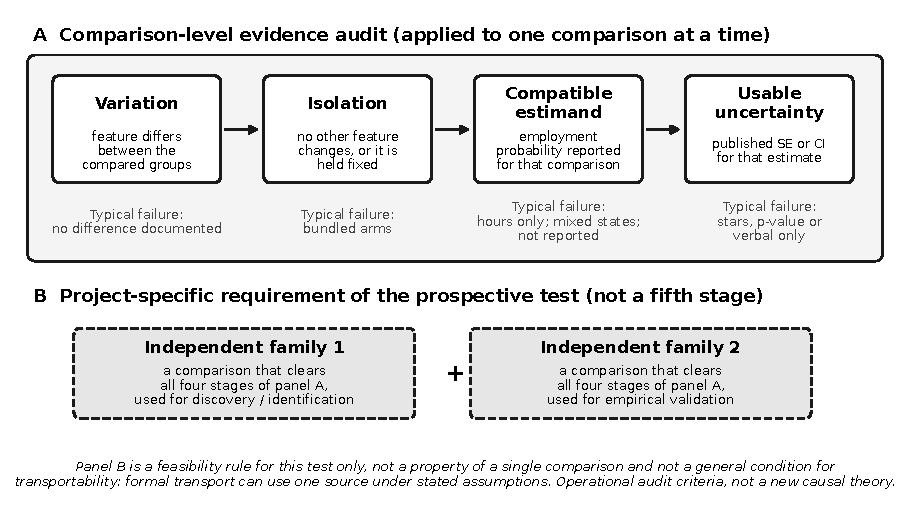
\includegraphics[width=\textwidth]{fig1_support_chain.pdf}
\caption{Comparison-level audit stages and the validation requirement for an empirically validated claim about one programme-design feature. The four stages---variation, isolation, compatible estimand and usable uncertainty---are evaluated on one comparison at a time. Independent validation, drawn separately, is not a fifth stage but a requirement of the prospective test considered in this paper (one family for discovery, one for validation); it is not a general definition of transportability, which can be identified from one source under stated assumptions. The stages are operational audit criteria, not a new causal theory.}
\label{fig:chain}
\end{figure}

\section{Evidence universe and prospectively specified rules}

The evidence universe has two layers with different roles (Table~\ref{tab:universe}).

\paragraph{Layer A} is a census of a frozen, frame-defined universe of 43 modern randomised basic-income, guaranteed-income and closely related experiments with employment outcomes. % N-01
It is not a census of every experiment of this kind: the frame was assembled from published reviews and frozen before extraction. Of the 43 frame members, 39 were verified against primary sources, 2 remained pending and 2 had unresolved frame conflicts; all were retained, and none of these four belongs to a strictly supported family. % F-01 N-01
Census statements, such as how many experiments vary a feature, refer to Layer A only.

\paragraph{Layer B} is an audit of 9 historical and adjacent designs, frozen before extraction because their published descriptions indicated design variation that the modern frame does not cover: the New Jersey-Pennsylvania \citep{watts1974}, rural \citep[RIME;][]{irp1976rime}, Gary \citep{kehrer1979} and Seattle-Denver \citep{riddell2024} negative-income-tax experiments, Canadian Mincome \citep{hum1993}, a long-term universal transfer in Kenya \citep{banerjee2023}, the Vermont \citep{scrivener2002} and Minnesota \citep{miller2000} welfare-reform experiments and a cash programme in northern Nigeria \citep{bastian2017}. % N-02
Layer B is not a census. Its role is to add support paths, especially isolated historical designs; no prevalence is computed over it, and the two layers are never pooled into a common denominator.

\paragraph{Target.} The outcome domain is employment, and the target estimand is the individual probability of being employed or working during treatment. We chose this extensive-margin target because it is policy-relevant and comparatively harmonisable across very different programmes, and we specified it before the census was coded. It is a target choice, not the only defensible one; Section~\ref{sec:infeasible} reports how the conclusion changes under a broader extensive-margin target. The coding rules, the same-comparison requirement and the independence criteria were frozen before any census count was computed. Rule clarifications that became necessary during extraction were adopted as general rules and re-applied to every case, never as case-specific exceptions (Methods).

% generated by scripts/build_manuscript_tables.py from SCOPE_C_FINAL_SUPPORT_GEOMETRY.csv, LAYER_B_SUPPORT_AUDIT.csv and RECONCILED_LAYER_A_MANIFEST.csv -- do not edit
\begin{table}[t]
\centering
\caption{Evidence universe. The two layers have different roles and are never pooled into a common denominator.}
\label{tab:universe}
\small
\begin{tabular}{@{}p{0.18\textwidth}p{0.37\textwidth}p{0.37\textwidth}@{}}
\toprule
 & Layer A & Layer B \\
\midrule
Definition & Census of a frozen, frame-defined set of modern basic-income, guaranteed-income and closely related randomised experiments with employment outcomes & Audited set of historical and adjacent designs with documented variation in programme design, frozen before extraction \\
Members & 43 experiments (frame status: 39 verified; 2 pending; 2 frame conflict; all retained) & 9 design cases \\
Status & Census of the frame (denominator for prevalence statements) & Audit (not a census; no prevalence is estimated) \\
Role & Census support geometry; selection audit & Additional support paths, especially isolated historical designs \\
Unit of independence & Transport family (independent identification source) & Transport family \\
\bottomrule
\end{tabular}

\smallskip
\parbox{\linewidth}{\footnotesize Layer B members: Feed the Future Nigeria Livelihoods Project cash; Gary NIT; GiveDirectly Kenya long-term UBI study; Mincome (Manitoba); Minnesota Family Investment Program; New Jersey-Pennsylvania NIT; Rural Income-Maintenance Experiment (RIME); Seattle-Denver Income Maintenance Experiment (SIME/DIME); Vermont Welfare Restructuring Project. Outcome domain: employment; prospectively specified target: individual probability of being employed or working.}
\end{table}


\section{The census geometry: where design support is lost}

Design variation is common in the census, and it is lost at identifiable stages (Figure~\ref{fig:attrition}, Table~\ref{tab:geometry}).

\paragraph{Withdrawal.} Of the 43 transport families, 9 vary the withdrawal schedule, 2 isolate it, and 1 of these reports a compatible employment estimand with usable uncertainty \citep{verlaat2025}. % N-03 N-01
Most varying withdrawal designs are bundled with other changes or their isolation is not established. A common pattern in Dutch municipal social-assistance experiments is to combine an earnings disregard with relaxed obligations in the same arm \citep{verlaat2022cpb}. One isolated design, in Wageningen, reports only an extensive-margin object defined by hours or earnings thresholds, which is not the prospectively specified target \citep{muffels2020}.

\paragraph{Conditionality and cadence.} For conditionality the counts are 7, 2 and 1; the strictly supported family is the Utrecht experiment \citep{verlaat2026}. % N-04
For payment cadence, 2 families vary and isolate the feature, 1 reports a compatible estimand, and none reports it with usable uncertainty. % N-05

\paragraph{Magnitude, duration and baseline state.} Transfer magnitude varies across 26 families and promised duration across 33. % N-06 N-07
Both vary almost entirely between studies, together with population, place, period and the rest of the programme, so they are never isolated within this census; associations between such study-level features and effects are observational \citep{thompson2002}. Their between-study support is nonetheless substantial: 6 families combine a measurable magnitude with a compatible employment estimate and usable uncertainty, and 6 do so for duration. % N-06 N-07
Baseline employment is a state descriptor rather than a policy feature; observed shares are available for 6 families, 2 of them with a compatible estimate and usable uncertainty. % N-08
The geometry also exposes measurement gaps. Normalised transfer magnitude cannot be established for 17 of the 43 experiments, mainly because baseline household income or the ex-ante transfer schedule is not reported, and baseline employment is unknown for 37. % N-19 N-01
We record these cells as unknown, not as absence of variation.

\begin{figure}[t]
\centering
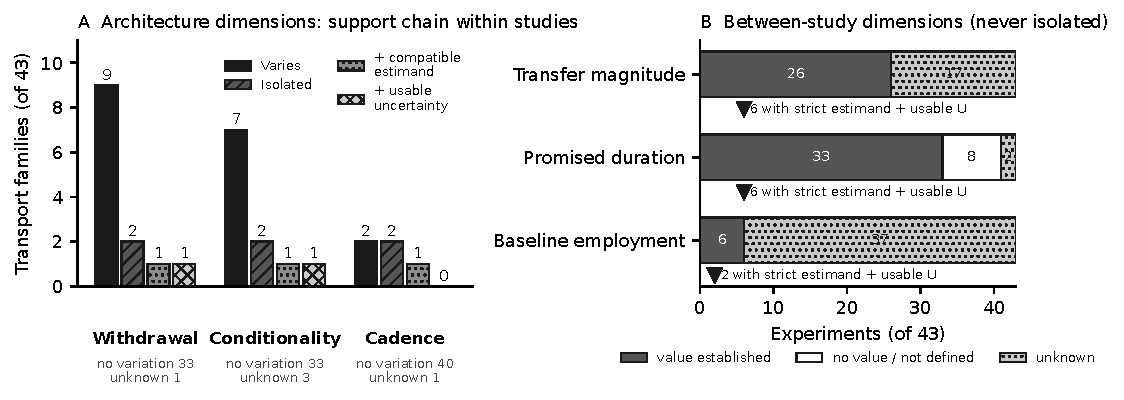
\includegraphics[width=\textwidth]{fig2_census_attrition.pdf}
\caption{Where design support is lost in the census of 43 frame-defined experiments. % N-01
 (A) Programme-design dimensions that can vary within a study: counts of transport families that vary the feature, isolate it, also report a compatible employment estimand and also report usable uncertainty; counts with no variation and with unknown status are given below each group. (B) Dimensions that vary only between studies and are never isolated: experiments with an established value, no value or unknown status; the marker gives the families that combine a value with a compatible estimand and usable uncertainty. No effect sizes are shown.}
\label{fig:attrition}
\end{figure}

% generated by scripts/build_manuscript_tables.py from SCOPE_C_FINAL_SUPPORT_GEOMETRY.csv -- do not edit
\begin{table}[t]
\centering
\caption{Support geometry by dimension. Entries are counts of transport families (independent identification sources) that vary the feature / isolate it / also report a compatible employment estimand / also report usable uncertainty (standard error or confidence interval).}
\label{tab:geometry}
\footnotesize
\setlength{\tabcolsep}{3.5pt}
\resizebox{\textwidth}{!}{%
\begin{tabular}{@{}lccccccl@{}}
\toprule
Dimension & Layer A census & Layer B audit & Support union & Between-study & Independent & Broader (E-B) & Support \\
 & (of 43) & (9 cases) & (not prevalence) & strict support & strict sources & isolated + U & stops at \\
\midrule
Transfer magnitude & 26/0/0/0 & 0/0/0/0 & 26/0/0/0 & 6 & 0 & 0 & isolation \\
Withdrawal schedule & 9/2/1/1 & 4/3/0/0 & 13/5/1/1 & 0 & 1 & 2 & estimand \\
Conditionality & 7/2/1/1 & 2/1/1/0 & 9/3/2/1 & 0 & 1 & 2 & uncertainty \\
Payment cadence & 2/2/1/0 & 1/1/1/0 & 3/3/2/0 & 0 & 0 & 0 & uncertainty \\
Promised duration & 33/0/0/0 & 2/1/0/0 & 35/1/0/0 & 6 & 0 & 0 & isolation \\
Baseline employment (state) & 6/0/0/0 & 0/0/0/0 & 6/0/0/0 & 2 & 0 & 0 & isolation \\
\bottomrule
\end{tabular}}

\smallskip
\parbox{\linewidth}{\footnotesize Layer A columns are census counts for the frame; the support union combines Layer A cells with Layer B audit paths and is not a prevalence. Magnitude, duration and baseline employment vary almost only between studies and are never isolated; their between-study support is shown separately. ``Broader (E-B)'' admits extensive-margin objects such as hours- or earnings-threshold employment; it is a sensitivity view, not the prospectively specified target. ``Support stops at'' is the stage at which the union loses support.}
\end{table}


\section{Selection dependence of the pre-census evidence set}

Before the census was built, the project worked with a smaller evidence set assembled for an earlier question about transfer magnitude. Seven of its experiments fall inside the census frame, so these 7 experiments are part of the 43. That set was not chosen to be biased, but sets built for one question tend to favour studies that report what that question needed. We therefore compared the 7 mapped experiments with the full census of 43 under identical rules (Figure~\ref{fig:selection}). % N-09

The mapped subset was strongly enriched for usable uncertainty. Between-study magnitude support with a compatible employment estimate and a standard error or confidence interval was present in 5 of the 7 mapped experiments but in only 6 of the 43 census experiments; % N-09
for duration, the corresponding figures are 4 of 7 and 6 of 43. % N-10
The full census added design variation in absolute terms: the number of families varying withdrawal grew from 3 to 9, conditionality from 2 to 7, and cadence from 1 to 2. % N-12
The added variation did not survive the later stages. Strictly supported isolated families were unchanged between subset and census: 1 and 1 for withdrawal, 1 and 1 for conditionality, 0 and 0 for cadence. % N-11

This answers a natural objection, that support appears scarce only because the wrong studies were examined. The opposite holds: moving from a purpose-built set to the frame-defined census increased design variation but not strictly supported evidence, and the earlier set had, if anything, looked better supported. Because the subset is nested in the census, the comparison is descriptive; no test statistic is computed.

\begin{figure}[t]
\centering
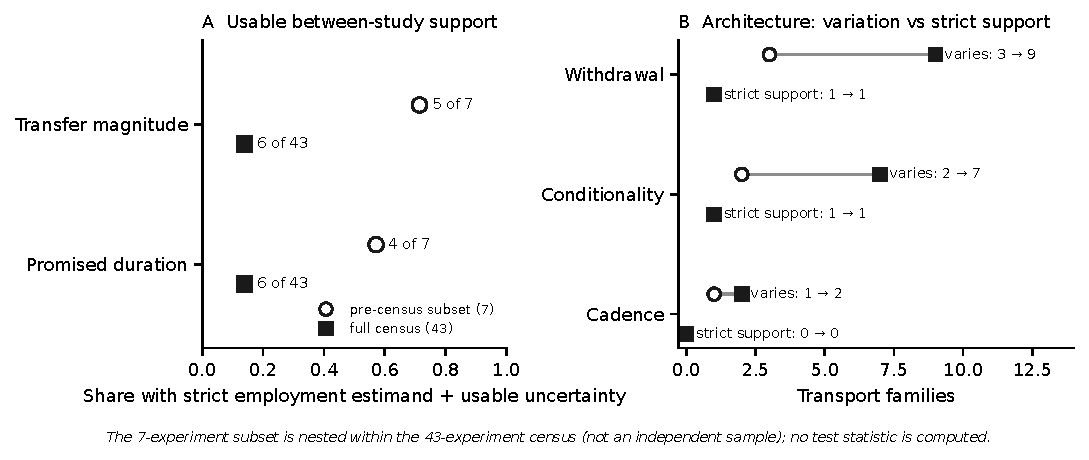
\includegraphics[width=\textwidth]{fig3_selection_audit.pdf}
\caption{Selection dependence of the pre-census evidence set. % N-09
The 7-experiment subset is nested within the 43-experiment census; it is not an independent sample, and no test statistic is computed. (A) Share of experiments with between-study support (compatible employment estimand and usable uncertainty) for transfer magnitude and promised duration. (B) Families varying each programme-design feature, and families passing every audit stage, in the subset and in the census.}
\label{fig:selection}
\end{figure}

\section{Historical and adjacent designs: isolation without validated evidence}

The audit layer adds designs that isolate design features more cleanly than most modern pilots. For withdrawal, 3 Layer-B families isolate the feature, each by randomising households to plans with the same guarantee and different withdrawal rates. % N-22
None of them supplies a compatible employment estimand with usable uncertainty for that focal comparison in its accessible record (Figure~\ref{fig:nearmiss}).

The Rural Income Maintenance Experiment (RIME), conducted in North Carolina and Iowa in the early 1970s, illustrates the gap. Families were randomised to 5 negative-income-tax plans or a control; in 3 pairs of plans the guarantee was identical and only the tax rate on income differed. % N-21
These same-guarantee, different-rate comparisons isolate the withdrawal schedule. The accessible published record reports employment as a comparison of all plans pooled against the control, by site and population group, and predictions from a regression that treats the guarantee and the tax rate as linear terms \citep{irp1976rime}. Neither is the focal comparison: the pooled contrast changes the guarantee and the tax rate together, and the regression predictions are model-based. No compatible published direct contrast was located in the accessible RIME-family record after the bounded search, and no standard errors or confidence intervals were located for any labour result in that record. The negative-income-tax experiments were designed to estimate labour-supply responses to the guarantee and the tax rate, and their analysts fitted response functions across plans; for the rural experiment, a secondary account reports that the standard errors of the response coefficients were large \citep{orrgubits2023}. Such model-based response-surface estimates are recorded here as model-only paths, which do not isolate a design contrast whatever uncertainty is reported for them. Several original technical volumes could not be accessed, so we do not conclude that the contrast was never estimated.

The New Jersey-Pennsylvania \citep{watts1974} and Gary \citep{kehrer1979} experiments show the same pattern: both have isolated withdrawal designs for which no compatible direct employment contrast with usable uncertainty was located in the sources read. In the Seattle-Denver experiment, withdrawal varies together with other features \citep{riddell2024}. Among the adjacent designs, the Vermont welfare-reform experiment provides an isolated conditionality contrast with a compatible employment estimate, reported with significance stars but without a standard error or interval \citep{scrivener2002}. Layer B therefore adds isolated variation and identification-capable designs, but not an independent source that passes every stage. Design availability, even in a well-randomised experiment, does not by itself provide validated cross-setting evidence.

\begin{figure}[t]
\centering
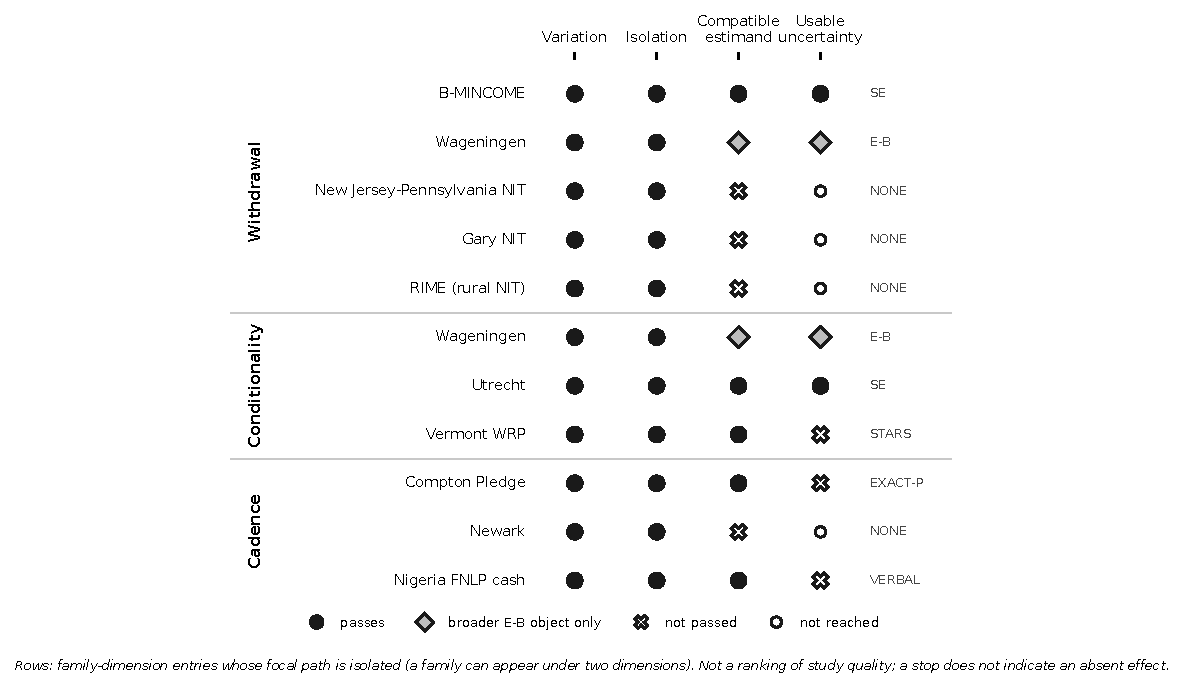
\includegraphics[width=0.86\textwidth]{fig4_near_miss_matrix.pdf}
\caption{Where isolated designs stop in the audit chain. Each row is one family--dimension entry: a transport family whose focal comparison on that dimension is isolated, grouped by dimension (a family isolated on two dimensions appears twice: Wageningen); markers show whether each stage is passed, passed only for a broader extensive-margin (E-B) object, not passed, or not reached, and the right-hand label gives the reported estimand or uncertainty form. The figure is not a ranking of study quality, and a stop does not indicate an absent effect. Sources: B-MINCOME \citep{verlaat2025}; Wageningen \citep{muffels2020}; New Jersey-Pennsylvania \citep{watts1974}; Gary \citep{kehrer1979}; RIME \citep{irp1976rime}; Utrecht \citep{verlaat2026}; Vermont \citep{scrivener2002}; Compton \citep{balakrishnan2024}; Newark \citep{tandon2025}; Nigeria \citep{bastian2017}.}
\label{fig:nearmiss}
\end{figure}

\section{Why a validated test of design-based prediction is currently infeasible}
\label{sec:infeasible}

Combining the census with the audit layer, the number of independent families passing every audit stage is 1 for withdrawal, 1 for conditionality, 0 for cadence and 0 for duration contrasts assigned within a study. % N-16
A prospective test of whether programme-design features predict employment responses across settings needs, for at least one dimension, one independent source for discovery and a second for validation. Within this frame-defined evidence universe, no programme-design dimension has two independent experiments that each report, for an isolated comparison, a compatible employment estimate with a published standard error or confidence interval. A prospectively specified discovery-and-validation test of design-based employment prediction therefore cannot currently be run; this is a statement about available evidence, not evidence that design features are unimportant. No such predictive test was run, and nothing here bears on its outcome. Adding the historical layer changed none of the dimension-level summaries. Transfer magnitude, which does have independent between-study support, was the subject of a separate, prospectively specified test of a simple magnitude-based summary within this project; that test did not support the summary, and we do not revisit it here.

\paragraph{The conclusion depends partly on the target.} The prospectively specified target counts only the probability of employment. If extensive-margin objects defined by hours or earnings thresholds were also admitted, withdrawal and conditionality would each have two supporting families, while cadence would still have none. % N-17
Both expanded pairs rely on the same Dutch municipal experiment, Wageningen. These broader objects are legitimate labour-market evidence; they are not the target specified in advance, and admitting them after seeing the counts would change the question in response to the data. We report the sensitivity because it shows that feasibility depends on outcome harmonisation. A future programme could adopt a broader target, but only prospectively and with its own rationale. The conclusion under the prospectively specified target is unchanged.

\section{What evidence would change the status?}

The blockers are specific enough to define the smallest evidence objects that would change the status of each dimension. Several existing designs could, in principle, supply them; we make no claim that the necessary data are currently accessible.

\paragraph{Withdrawal (support stops at the estimand).} One family passes every stage. Isolated same-guarantee designs exist in RIME, New Jersey-Pennsylvania and Gary, but in their accessible records the focal employment contrast is not reported in compatible form. The missing object is a direct same-rule employment estimate with a standard error or confidence interval from one additional independent family. For RIME the design is suitable in principle, but the accessible published record is insufficient and a data-access route has not been established. A new experiment varying only the withdrawal rate at a fixed guarantee would also suffice.

\paragraph{Conditionality (support stops at uncertainty).} One family passes (Utrecht). The Vermont experiment has an isolated contrast with a compatible employment estimate reported only with significance stars. A valid standard error or interval for that focal contrast, produced under an appropriate prospective protocol, would create the second family; this is the smallest gap in the evidence base.

\paragraph{Cadence (support stops at uncertainty).} The Compton Pledge reports a compatible employment comparison of payment schedules with an exact p-value only \citep{balakrishnan2024}; the Nigerian cash programme reports a verbal result only \citep{bastian2017}; and the Newark experiment varies cadence cleanly but reports no focal employment result \citep{tandon2025}. Two independent cadence families with standard errors or confidence intervals are needed, for example usable uncertainty for both the Compton and the Nigerian designs.

\paragraph{Duration (support stops at isolation).} Promised horizons vary widely across studies, but cross-study variation is not isolated causal evidence about duration. The designs that assign different horizons within a study report hours or non-employment outcomes. Status-changing evidence would be assigned horizon contrasts with comparable design, employment estimands and usable uncertainty in two independent families.

\paragraph{Transfer magnitude and baseline employment.} The simple magnitude summary has already been tested and not supported; we do not propose further magnitude studies to revisit it. Future trials can usefully supply consistent measurement of baseline household income and the ex-ante transfer. Baseline employment is a state descriptor; reporting it consistently would improve future analyses but does not identify any design effect.

Several gaps concern reporting rather than design. Box~1 summarises the minimum reporting that would have prevented the losses observed here; the full version, with the blockers each item addresses, is in the Supplementary Information. It is minimum reporting for transport and compression analysis of programme design, not a universal reporting standard for randomised trials, and it complements the established recommendation to estimate interactions from within-study information \citep{riley2020}.

\begin{center}
\fbox{\parbox{0.93\textwidth}{\small
\textbf{Box 1. Minimum reporting for analysis of programme design across settings}
\begin{enumerate}
\item Full arm-specific design: transfer rule, withdrawal schedule, conditions, cadence, promised horizon and services.
\item Assignment counts and the analysed population relative to the assigned sample.
\item Direct, pre-specified arm-against-arm contrasts for each varied feature, with covariance when arms share a control.
\item Exact definitions of the employment states counted as positive and negative.
\item A focal estimate with a standard error or confidence interval, not only a p-value or stars.
\item Baseline income and employment inputs, implementation differences, and machine-readable results or a data-access route.
\end{enumerate}}}
\end{center}

\section{Discussion}

\paragraph{What is established.} Within this evidence universe and for employment, design variation is common; strictly supported evidence about programme design is sparse; the scarcity survives expansion from a purpose-built evidence set to the frame-defined census; historical designs add isolation but not an independent pair; and support is lost at different stages for different dimensions---isolation and the estimand for withdrawal, uncertainty for conditionality and cadence, isolation for duration. These are statements about the published and accessible evidence structure.

\paragraph{What is not established.} This paper does not test whether basic income or any of its features affects employment, and it does not bear on whether basic income is desirable policy. It does not show that design features are unimportant, and it does not refute any general representation of programme design: the test was not feasible, so it was not run. Nor does it establish that other policy literatures share this geometry. That a literature can be rich in trials and poor in evidence that isolates and validates mechanisms is a plausible hypothesis for other fields, which this single audit does not test.

\paragraph{Relation to prior work.} For the negative-income-tax experiments, \citet{burtless1986} observed that pooled responses mixed different plans and populations, that within-experiment guarantee and tax-rate effects were confounded by stratified assignment and imprecisely reported, and that applying estimates to other settings depended on the reference welfare system; \citet{elmore1986} described experimental treatments as packages whose untested variants required extrapolation. Our historical audit confirms and updates these diagnoses rather than discovering them. For modern cash transfers, \citet{crosta2024} note that meta-analysis relies largely on cross-study variation and run formal moderator analyses that we do not attempt; \citet{bastagli2016} document collinearity among programme features; \citet{chrisp2022} code the designs of experiments in high-income countries without linking design to outcomes; and \citet{corinth2026} document incompatible employment definitions across recent guaranteed-income pilots. The general difficulties---transport under assumptions, compound treatments and the observational character of between-study moderators---are standard \citep{pearl2014,degtiar2023,hernan2011,thompson2002}. \citet{orr2026} asks whether evidence that an intervention is effective gives sound advice to a locality deciding whether to adopt it; the question here arises when a policymaker must instead choose the architecture of a basic-income programme, and asks whether the experimental literature contains identified and reported evidence about the relevant design dimensions. The gap emphasised by \citet{doussard2026}, community and general-equilibrium effects, is distinct from and complementary to the individual-level design evidence audited here. What this paper adds is a reproducible decomposition that is complete within the frozen frame, counted by independent source, together with a quantitative selection audit and a research agenda derived mechanically from the observed blockers.

\paragraph{Analytical recoverability.} The agenda distinguishes three situations: an experimental design exists; its focal result is reported; and the data needed to construct the focal result prospectively are practically recoverable. We use the term analytical recoverability, descriptively, for the degree to which an existing design can be reused to construct the required estimate and uncertainty from accessible reporting or legally obtainable data. It is an interpretation of the agenda, not an additional audit stage. Some existing experiments may be difficult to reuse because the focal result is unreported, uncertainty was incompletely reported, historical material is not publicly accessible, or the necessary data are not practically recoverable without institutional and data-security infrastructure. Where an existing randomised design already isolates the feature, making it analytically reusable may sometimes add more to validated cross-setting knowledge than another loosely targeted pilot would. This is a statement about the structure of the evidence gap, not a cost comparison.

\section{Limitations}

\begin{enumerate}
\item \textbf{Outcome domain.} Employment is the focal domain; hours, earnings, health and other outcomes may show a different geometry.
\item \textbf{Target choice.} The employment target was chosen in advance; a broader extensive-margin target would strengthen support for two dimensions (Section~\ref{sec:infeasible}).
\item \textbf{Frame.} Layer A is a census of a frozen frame, not of every relevant experiment; Layer B is an audit of designs chosen for their variation, not a census, and is not exhaustive.
\item \textbf{Prior-art search.} The prior-art audit was bounded and identified five sources that could not be read because of access or retrieval barriers. We do not characterise their content and do not treat their inaccessibility as evidence of absence of precedent; novelty claims are therefore deliberately narrow.
\item \textbf{Reporting is not evidence.} Absence of a reported result is not absence of underlying evidence; unpublished analyses or inaccessible reports may contain some of the missing objects, and some source searches were bounded by access.
\item \textbf{Coding.} The blinded second coding pass covered 25 cases from the pre-census evidence map, not the whole census; agreement on the estimand code was materially weaker than on variation, isolation and uncertainty; three rules adopted after that exercise were re-applied globally but were not independently second-coded; and much of the census extraction was carried out by a single coding process. % REL
\item \textbf{No effects tested.} The audit evaluates evidence support; it does not estimate or test policy effects.
\end{enumerate}

\section{Conclusion}

The basic-income and guaranteed-income literature does not lack experiments. What it currently lacks for empirically validated cross-setting claims about programme design is a small number of specific evidence objects: direct same-rule contrasts, harmonised employment estimands, usable uncertainty, and independent replication of the same comparison. Because these objects are specific---one more independent withdrawal contrast meeting every stage, usable uncertainty for an existing isolated conditionality contrast, two independent cadence contrasts---future progress can be judged against explicit status-changing requirements rather than against the number of trials.

\section*{Methods}

\paragraph{Evidence universe.} Layer A was defined by a frame of modern randomised basic-income, guaranteed-income and closely related experiments with employment outcomes, assembled from published reviews used as locators \citep{chrisp2022,corinth2026}. Membership was frozen before any study was coded, and every frame member was retained in the denominator of 43, including members whose verification remained pending or conflicted. % N-01
Layer B was frozen at the same time: 9 historical and adjacent experiments selected because their design descriptions indicated variation in withdrawal, conditionality, payment profile or promised duration. % N-02
Layer B is analysed as a set of support cases; no prevalence statement is made about it.

\paragraph{Extraction.} For each frame member, the extraction recorded from the study's own primary sources the programme identity and sites; the assignment mechanism, randomisation unit and strata; the assigned arms with their transfer rules, withdrawal schedules, obligations, payment frequency, promised horizon and services; the contrasts defined by the design; and every located employment-related result, with its exact positive and negative states, analysis sample, horizon and published inferential information. Identity checks were run before aggregation, to avoid counting one experiment twice or merging distinct experiments that share a programme label. Where two primary sources disagreed on a design parameter, both versions were kept and the field marked unresolved, unless a documented source hierarchy justified a choice. Secondary reviews were used as locators only; searches for each study's source family were bounded and logged, and inaccessible sources were recorded as such and not circumvented.

\paragraph{Units.} Each experiment was assigned to a statistical dependence group, which links estimates sharing samples or assignment, and to a transport family, which links sources sharing the identifying variation. Arms and sites of one coordinated experiment belong to one family. Experiments sharing only an evaluator, sponsor, era or design tradition were kept as separate families when their samples, sites and assignment were distinct; families whose independence could not be established were never counted toward an independent pair.

\paragraph{Coding.} For each experiment and each of six dimensions---transfer magnitude, withdrawal schedule, conditionality, payment cadence, promised duration and baseline employment---the comparisons defined by the design were coded for variation (yes, no, unknown); isolation (pure; conditionable bundle, where another feature changes but the design holds it fixed; bundled; not isolated, between-study only; or model-only); estimand compatibility (employment probability, with or without a documented definitional caveat; another extensive-margin object; another labour outcome such as hours or earnings; or none); and uncertainty form (standard error; confidence interval; exact p-value; test statistic; p-value category; stars; verbal; or none). Consequences that follow mechanically from the focal feature were not treated as co-interventions; documented research-procedure differences between arms, such as participation payments for one arm only, were. A positive state that could be satisfied through a non-labour state, or a label whose state definition was not established, was excluded from the employment domain. A design capable of identifying an effect was never treated as a reported result, and normalised magnitude was recorded as unknown when its inputs were not reported, never imputed from post-treatment payments.

\paragraph{Outcome domain and same-comparison rule.} Support cases are indexed by outcome domain: an estimate on hours or earnings can support a case in that domain but is never copied into an employment case. Within the employment domain, each support case is anchored to one comparison, so a family is never credited with the isolation of one contrast combined with the estimate or uncertainty of another. When a design defines several comparisons for the same dimension, every eligible comparison is kept, and a family passes a stage only if one comparison passes that stage and all preceding stages.

\paragraph{Gates and counts.} The strict path requires, on the same comparison, variation; isolation (pure or conditionable bundle); a compatible employment estimand; and a published standard error or confidence interval. No uncertainty was derived from p-values, test statistics or stars, and standard errors from separate arm-against-control comparisons were never combined into an arm-against-arm comparison; this is a conservative reporting rule, not a claim that such information carries no uncertainty. A broader extensive view, reported only as a sensitivity analysis, also admits extensive-margin objects. Counts are numbers of distinct transport families. Between-study dimensions are summarised separately by the number of families with a measurable value and a compatible estimate with usable uncertainty. Dimension-level qualitative summaries are given in the Supplementary Information.

\paragraph{Selection audit.} The 7 census experiments that had been mapped before the census was built were compared with the full census under identical rules and family counting. % N-09
Because the subset was assembled for a different question and is nested in the census, the comparison is descriptive and diagnostic of selection, not of intent.

\paragraph{Prospective specification.} The coding rules, the employment target and the independence criteria were specified before the census was extracted and frozen before any census count was computed. These freezes were internal, dated and hashed; there was no external public preregistration. Ambiguities discovered during extraction were resolved by general rule clarifications, adopted before aggregation, re-applied to every case and recorded with their trigger---never by case-specific exceptions, and never by reference to whether a resolution would change the feasibility result. Effect signs and magnitudes were not used at any stage of coding, comparison selection or aggregation.

\paragraph{Blinded second coding pass.} Before the census was extracted, a blinded second coding pass, carried out separately from the original coding and without access to the original codes, coded 25 support cases using only the frozen codebook, the coding protocol and blinded case packets. Pre-adjudication agreement was: variation 25 of 25 (kappa undefined, all codes identical); isolation 23 of 25 (0.92; Cohen's kappa 0.884); estimand, exact codes, 19 of 25 (0.76; kappa 0.490); estimand with the two employment-probability classes merged, 21 of 25 (0.84; kappa 0.606); uncertainty 24 of 25 (0.96; kappa 0.936); usable-uncertainty flag 24 of 25 (0.96; kappa 0.918). % REL
Both the original coding and the second pass were performed by AI systems (see AI use and author responsibility), so these statistics are inter-coding reproducibility diagnostics for the written codebook, not conventional inter-rater reliability between human coders. The estimand code was the weak point: two original estimand classifications for withdrawal designs were found on adjudication to credit a compatible estimand that the sources did not report, which moved two families out of the compatible-estimand stage and materially changed the withdrawal geometry. Disagreements were resolved by general codebook clarifications re-applied to all cases; post-adjudication agreement is not reported as reliability. Three rules introduced after this exercise---on mixed labour and non-labour states, outcome-definition sufficiency and research-procedure co-interventions---were re-applied globally but were not independently second-coded, so the census was not independently double-coded in full.

\paragraph{Construction and reproducibility.} All counts and tables are produced by deterministic scripts from frozen coded tables that contain support codes but no effect estimates. Automated checks recompute every count and confirm the gate logic and family counting (Supplementary Information). No participant-level data were used.

\section*{GenAI use disclosure}
The evidence coding and repository implementation used AI-assisted workflows under the author's direction. 
The original support coding, the master evidence map, the operational text of the codebook and the census extraction 
were produced by the project's Claude Code agent (Claude Opus 5.5), implementing scientific rules and specifications 
that the author defined and revised. 
The blinded second coding pass of 25 cases was performed by GPT-5.6 Sol in a separated context-free session, with access 
only to the blinded materials described in Methods and not to the original codes. % REL
Disagreements were adjudicated with AI assistance under the author's scientific oversight and final decision authority, 
and the resulting codebook clarifications were implemented in the repository by Claude Code. 
ChatGPT (GPT-5.6 Sol) was used for interactive methodological reasoning and critique, review of the evidence architecture, 
development of coding rules and preparation of implementation instructions for the Claude Code agent. 
Google Gemini 3.1 Pro served as independent critique and adversarial stress-tester. 
The manuscript was drafted and edited with assistance from ChatGPT and Claude, and the analysis, build and validation code was 
generated and modified with substantial assistance from Claude Code. 
The author was responsible for the scientific design and coding rules, reviewed and accepted or rejected all AI-generated outputs, 
made all final scientific decisions and is responsible for the content of this article. 
No participant-level data were processed by any AI system.

\section*{Funding}
This research received no external funding.

\section*{Competing interests}
The author declares no competing interests.

%\section*{Author note}
%This research was conducted independently in the author's personal capacity. Ericsson AB did not sponsor, fund, commission, supervise or participate in the research, and the views expressed are those of the author alone.

\section*{Data and code availability}
The coded evidence tables, the frozen coding manual and the scripts that produce all counts, tables and figures are available in a public replication repository, \url{https://github.com/diazmendez/basic-income-design-evidence} (release v1.0.1), under the MIT licence for code and CC BY 4.0 for the coded data and documentation. That repository is a derived snapshot of the project's private working repository, and the corresponding private commit is recorded in the release. The repository has no archival deposit or DOI. The audit used only published or publicly accessible reports and coded study-level metadata. Third-party primary documents are cited and not redistributed, and restricted-access data were not used. No participant-level data are distributed by this project.

\bibliographystyle{plainnat}
\bibliography{references}

\end{document}
